
\begin{figure}[H]
	\centering
	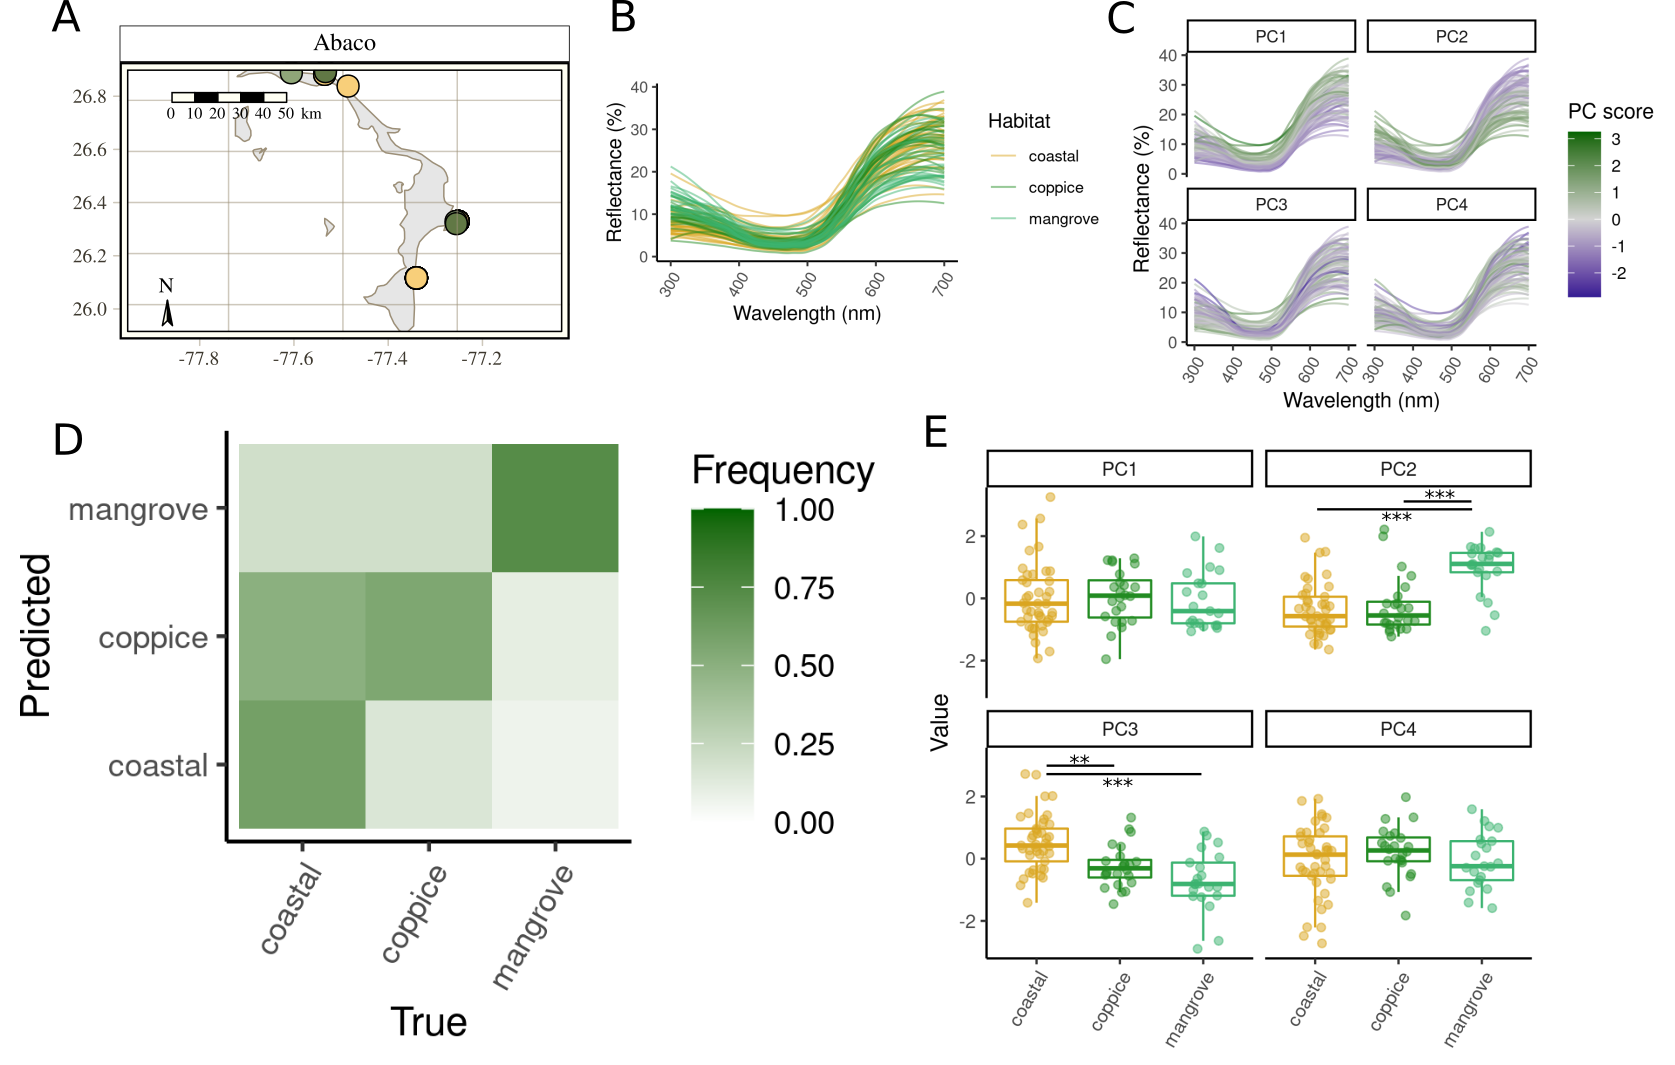
\includegraphics[width=\textwidth]{figures/Abaco.png}
	\caption{Comparison of dewlap coloration across habitats on Abaco. (A) Confusion matrix showing the proportion of lizards from each (true) habitat reassigned to each (predicted) habitat by the random forests, based on the first four within-island principal components and averaged across replicates. Each column sums to one. (B) One-dimensional sensitivity analysis showing the relative importance (mean decrease in accuracy) of the various wavelengths in random forest classification of the whole spectrum. (C) Reflectance profiles of all the dewlaps on the island. (D) Within-island principal component scores across habitats. Bars indicate significant contrasts. *, $P < 0.05$; **, $P < 0.01$; ***, $P < 0.001$. (E) How reflectance profiles map onto the within-island principal components. (F) Map of the island with the sampling sites colored by habitat. (G) Geographical distance between sites where significant differences were detected in within-island principal component scores (Wilcoxon test, Benjamini-Hochberg correction, $P < 0.05$), including only pairs of sites whose habitats were involved in between-habitat dewlap differences.}
	\label{fig:Abaco}
\end{figure}